\documentclass[11pt,a4paper]{article}
\usepackage{tikz}
\usetikzlibrary{arrows.meta,positioning}
\usepackage{tabularx}
\usepackage{amsmath,amssymb,amsthm}
\usepackage{geometry}
\geometry{margin=1in}
\usepackage{hyperref}
\usepackage{graphicx}
\usepackage{setspace}
\onehalfspacing

\title{\textbf{Paper C-09: Socioeconomic Crises:\\ A Constraint-Driven Flux Dynamics (CDFD) Perspective}}
\author{Steve Bico Mujjabi, MD\\
\small Independent Researcher\\
\small Founder, Vura Labs\\
\small Kampala, Uganda\\
\small ORCID: 0009-0001-0556-5516}
\date{August 2026}

\begin{document}
\maketitle

% BEGIN SHARED-METHODS POINTER
\noindent\textit{Shared Part IV notation and evidence boundaries are defined in \path{PART_IV_METHODS_AND_CLAIM_BOUNDARY.md}. This paper states only its local observables, comparison, and failure conditions.}
% END SHARED-METHODS POINTER


\begin{abstract}
This paper develops a falsifiable CDFD/AFL model of Socioeconomic Crises. It maps economic, political, ecological, health, and information shocks to driving flux $\Phi$, fiscal, liquidity, institutional, social, and household buffers to active constraint $C$, relief, coordination, substitution, learning, and collective action to responsiveness $S$, and debt, trauma, distrust, depleted assets, and prior crises to structural memory $M_s$. The target outcome is loss, unrest, contagion, recovery, and institutional change, tested against crisis chronologies, balance sheets, surveys, prices, policy actions, and recovery data. The paper treats universality as a shared model architecture rather than an assertion that unlike systems have the same material mechanism. It states the negative result that would make the mapping unnecessary and places the domain claim inside the cumulative CDFD programme and its reproducible runtime boundary.
\end{abstract}

\section{Introduction}

Complex human societies are highly ordered structures that require continuous inputs of energy, capital, and information to maintain their low-entropy state. To manage this massive throughput, societies construct institutions, laws, and bureaucracies. Over time, these regulatory mechanisms accumulate.

In the CDFD ontology, these bureaucracies represent systemic memory ($M_s$) and structural constraint ($C$). While necessary for initial stability, the runaway accumulation of these factors pushes the society toward an unstable topological edge.

\section{The Dynamics of Institutional Collapse}
We evaluate the systemic health of a civilization using the Adaptive Operating Ratio:
\begin{equation}
    \Psi_s = \left( \frac{\Phi}{C} \right) \cdot S \cdot M_s
\end{equation}

As an empire or state matures, its institutions become deeply entrenched. The legal code expands, trade tariffs multiply, and bureaucratic friction increases. In CDFD terms, the constraint $C$ and the memory $M_s$ grow monotonically.

To maintain a functioning society ($\Psi_s \approx 1$), the state must continuously increase its raw throughput $\Phi$ (e.g., through conquest, resource extraction, or technological innovation) to offset the rising constraints. If the state exhausts its external resources, $\Phi$ plateaus while $C$ continues to climb.

The adaptive ratio crashes: $\Psi_s \ll 1$. The society enters a state of systemic necrosis.

\subsection{The Mathematics of Revolution}
When a biological tissue drops into $\Psi_s \ll 1$, cells undergo apoptosis to shed constraint and salvage the organism. When a plasma drops into $\Psi_s \ll 1$, it undergoes magnetic reconnection to violently reset its topology.

When a human society drops into $\Psi_s \ll 1$, the populace (which retains high local responsiveness $S$) realizes that the central institutional constraints ($C$) are actively suffocating survival. Because the state's memory ($M_s$) is locked, peaceful, incremental reform is mathematically impossible.

The only viable topological solution is a sudden, violent reset of the constraints. This is a \textbf{Revolution} or \textbf{Collapse}. The central government is dissolved, instantly dropping the institutional constraint $C$ to near zero. The systemic memory $M_s$ is violently wiped (laws rewritten, debts cleared). The unified macro-surface fragments into smaller, localized nodes that can individually achieve a healthy $\Psi_s \approx 1$ equilibrium.



\section{Measurement Layer}

% BEGIN PART IV MAJOR CROSS-DOMAIN UPGRADE
\section{Cross-Domain Model Upgrade: Mechanism, Scale, and Tests}

\subsection{Observable Translation}

The paper-specific translation begins with an observable chain rather than a
verbal analogy. For Socioeconomic Crises, the proposed drive is economic, political, ecological, health, and information shocks.
The active limitation is fiscal, liquidity, institutional, social, and household buffers. Responsiveness is carried by
relief, coordination, substitution, learning, and collective action, while retained state is represented by
debt, trauma, distrust, depleted assets, and prior crises. The outcome to explain is loss, unrest, contagion, recovery, and institutional change.

\begin{table}[htbp]
\centering
\small
\caption{Operational CDFD/AFL map for Paper C-09.}
\begin{tabularx}{\textwidth}{|l|X|X|}
\hline
\textbf{Term} & \textbf{Paper-specific observable meaning} & \textbf{Measurement question} \\
\hline
$\Phi$ & economic, political, ecological, health, and information shocks & What rate, load, gradient, or demand enters the focal system? \\
\hline
$C$ & fiscal, liquidity, institutional, social, and household buffers & Which measured bottleneck limits transfer, function, or recovery? \\
\hline
$S$ & relief, coordination, substitution, learning, and collective action & Which process changes effective capacity or reroutes the load? \\
\hline
$M_s$ & debt, trauma, distrust, depleted assets, and prior crises & Which retained state makes equal present loads produce different futures? \\
\hline
$Y$ & loss, unrest, contagion, recovery, and institutional change & Which outcome is predicted out of sample, with uncertainty? \\
\hline
\end{tabularx}
\end{table}

\begin{figure}[htbp]
\centering
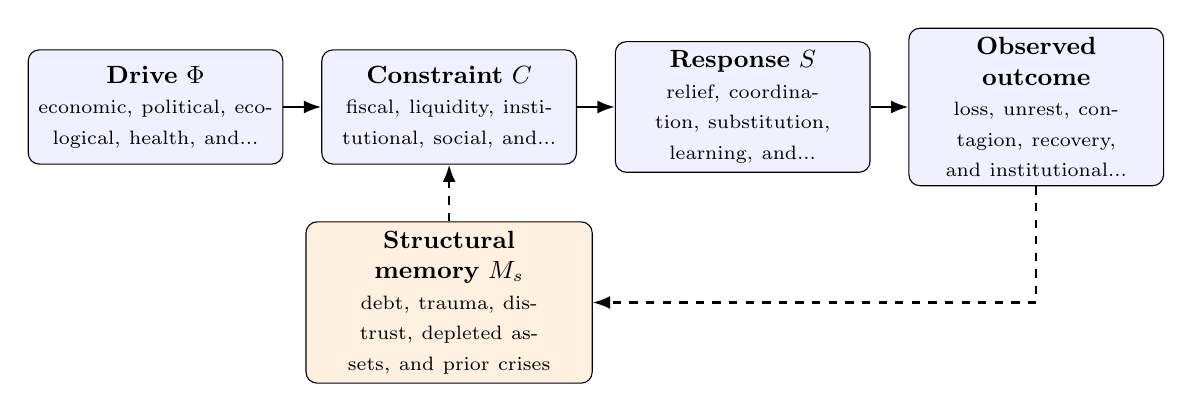
\begin{tikzpicture}[
    node distance=0.48cm,
    every node/.style={font=\small},
    box/.style={draw, rounded corners, align=center, minimum height=1.45cm, text width=3.0cm, fill=blue!6},
    memory/.style={draw, rounded corners, align=center, minimum height=1.25cm, text width=3.4cm, fill=orange!12},
    flow/.style={-{Latex[length=2.2mm]}, thick},
    feedback/.style={-{Latex[length=2.2mm]}, thick, dashed}
]
\node[box] (drive) {\textbf{Drive $\Phi$}\\\scriptsize economic, political, ecological, health, and...};
\node[box, right=of drive] (constraint) {\textbf{Constraint $C$}\\\scriptsize fiscal, liquidity, institutional, social, and...};
\node[box, right=of constraint] (response) {\textbf{Response $S$}\\\scriptsize relief, coordination, substitution, learning, and...};
\node[box, right=of response] (outcome) {\textbf{Observed outcome}\\\scriptsize loss, unrest, contagion, recovery, and institutional...};
\node[memory, below=0.72cm of constraint] (memory) {\textbf{Structural memory $M_s$}\\\scriptsize debt, trauma, distrust, depleted assets, and prior crises};
\draw[flow] (drive) -- (constraint);
\draw[flow] (constraint) -- (response);
\draw[flow] (response) -- (outcome);
\draw[feedback] (outcome.south) |- (memory.east);
\draw[feedback] (memory.north) -- (constraint.south);
\end{tikzpicture}
\caption{Paper C-09 observable CDFD/AFL architecture for Socioeconomic Crises. Solid arrows give the proposed forward chain; dashed arrows make history-dependent feedback explicit.}
\label{fig:c09-architecture}
\end{figure}

\subsection{Paper-Specific Causal Hypothesis}

For this paper, the hypothesized causal sequence is specific. A change in
economic, political, ecological, health, and information shocks arrives faster than relief, coordination, substitution, learning, and collective action can compensate.
This raises or redistributes fiscal, liquidity, institutional, social, and household buffers. If the load persists,
the retained state encoded by debt, trauma, distrust, depleted assets, and prior crises changes the next response, so a later event of equal
magnitude can produce a different trajectory in loss, unrest, contagion, recovery, and institutional change. The
scientific task is to estimate that sequence against the best ordinary model of
the domain, not merely to redescribe the outcome after it occurs.

\subsection{Cross-Scale Translation Without Mechanistic Erasure}

For the socioeconomic systems family, the cross-domain translation compares human and institutional throughput, unequal access to capacity, adaptive coordination, and historical path dependence. The variables are not morally neutral: aggregation can hide who receives flow, who bears constraint, and whose prior losses become persistent memory. \cite{BarabasiAlbert1999,WattsStrogatz1998,Holling1973,Shannon1948}
The required scale declaration for this paper is minutes to generations; households to international systems. At short
scales, the key question is whether the incoming drive is transmitted,
buffered, or diverted. At intermediate scales, response changes effective
capacity and network exposure. At long scales, retained structure can alter the
state space itself. A result is genuinely cross-scale only when the aggregation
rule is stated and the same conclusion is not an artifact of averaging.

\subsection{Evidence Ladder and Discriminating Tests}

\begin{table}[htbp]
\centering
\small
\caption{Evidence ladder for Paper C-09. Each rung can fail independently.}
\begin{tabularx}{\textwidth}{|p{0.17\textwidth}|X|X|}
\hline
\textbf{Test} & \textbf{Design} & \textbf{Discriminating result} \\
\hline
Proxy audit & Measure crisis chronologies, balance sheets, surveys, prices, policy actions, and recovery data and preregister how each record maps to $\Phi$, $C$, $S$, $M_s$, and $Y$. & The mapping fails if proxies are non-identifiable, circular, or change meaning across cases. \\
\hline
Load ramp & Apply or observe a repeated shock before full social or economic recovery while estimating the dominant constraint and response time. & A threshold claim requires a reproducible nonlinear change and uncertainty bounds, not a visually chosen breakpoint. \\
\hline
Recovery and memory & Match present load across units with different histories, then compare recovery paths. & The memory claim requires history-dependent divergence after current conditions are controlled. \\
\hline
Model comparison & Compare the baseline domain model with and without the CDFD/AFL state variables using held-out data. & The paper's stated falsifier is: prior-crisis memory does not alter severity or recovery after present exposure is matched. \\
\hline
\end{tabularx}
\end{table}

\subsection{Research Programme and Boundary Conditions}

The immediate research programme has four steps. First, construct a documented
dataset from crisis chronologies, balance sheets, surveys, prices, policy actions, and recovery data and retain raw units before normalization.
Second, fit a baseline domain model and report its calibration and out-of-sample
error. Third, add the smallest identifiable CDFD/AFL state extension and test
whether it improves prediction of loss, unrest, contagion, recovery, and institutional change. Fourth, repeat the
analysis across the declared scale range and publish negative cases as part of
the cross-domain translation audit.

% END PART IV MAJOR CROSS-DOMAIN UPGRADE

\section{Conclusion}
Socioeconomic collapse is the macro-scale equivalent of cellular necrosis or a stellar supernova. It is the physics of a system forced to violently shed its accumulated constraints and memory in order to restore the free flow of energy and information. CDFD provides a candidate measurable boundary for when political reform becomes impossible and systemic collapse risk rises.
\section*{Conflict of Interest} The author declares no conflict of interest.
\section*{Data Availability}
Part-specific runtime diagnostics are under each Part's \path{outputs/} directory.

Release-wide code: \path{Part_E_Synthesis/supplementary/}.

Generated summaries: \path{Part_E_Synthesis/outputs/}.

Figures: \path{Part_E_Synthesis/figures/}.


\section{Reference Layer}
\bibliographystyle{plain}
\bibliography{universal_afl_references}
\end{document}
